The deterministic event-based calculator is capable of computing losses and loss statistics for a single event for a collection of assets. Depending of the type of hazard input that is provided, two separate approaches can be followed. In the first one, the calculator uses two maps, one with the distribution of the mean ground motion and a second one with the associated aleatory variability. In the second approach, the event is repeated many times to model the variation in the inter-event variability and for each event, a ground motion field is generated taking into account the intra-event variability (and possibly the spatial correlation of the latter). The following scheme presents the architecture of this calculator:

\begin{figure}[ht]
\centering
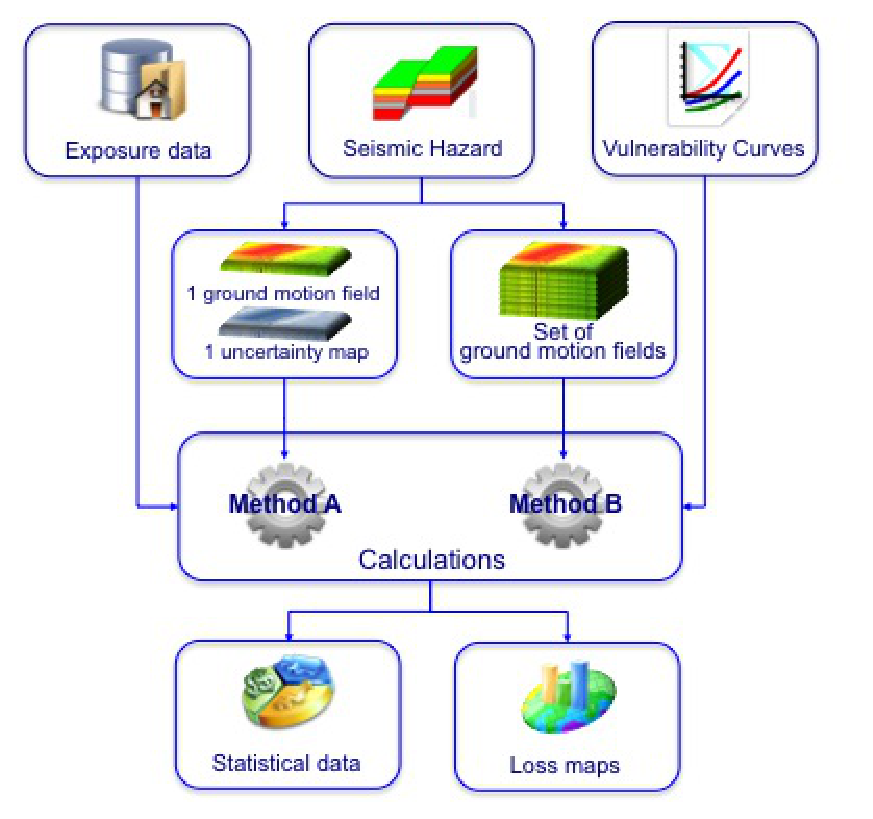
\includegraphics[width=9cm,height=9cm]{./Figures/Part_Risk/Scheme_Deter_calc.eps}
\caption{Architecture of the deterministic event-based calculator.}
\label{fig:Scheme_deter_calc}
\end{figure}

\section{Method A} 
\subsection{Description}
In this approach, after providing the two aforementioned maps, the mean ground motion and coefficient of variation at each site are used together with the assigned vulnerability function for each asset  to calculate a mean loss ratio. The aleatory variability in the ground motion is combined with the uncertainty in the vulnerability functions through the total probability theorem in order to calculate the standard deviation of the loss ratio for each asset.

\subsection{Calculation workflow}

To compute the mean loss:

\begin{enumerate}
\item In order to compute the probability of occurrence of each intensity measure level defined on the vulnerability function, an upper and lower bound needs to be calculated for each value. The limits for an $IML_n$ can be given by the following formulae:

\begin{equation}
Lower bound = \frac{IML_n+IML_{n-1}}{2}
\end{equation}

\begin{equation}
Upper bound = \frac{IML_{n+1}+IML_{n}}{2}
\end{equation}

The following figure illustrates the intervals that were computed based on 4 intensity measure levels that comprise a given vulnerability function:

\begin{figure}[ht]
\centering
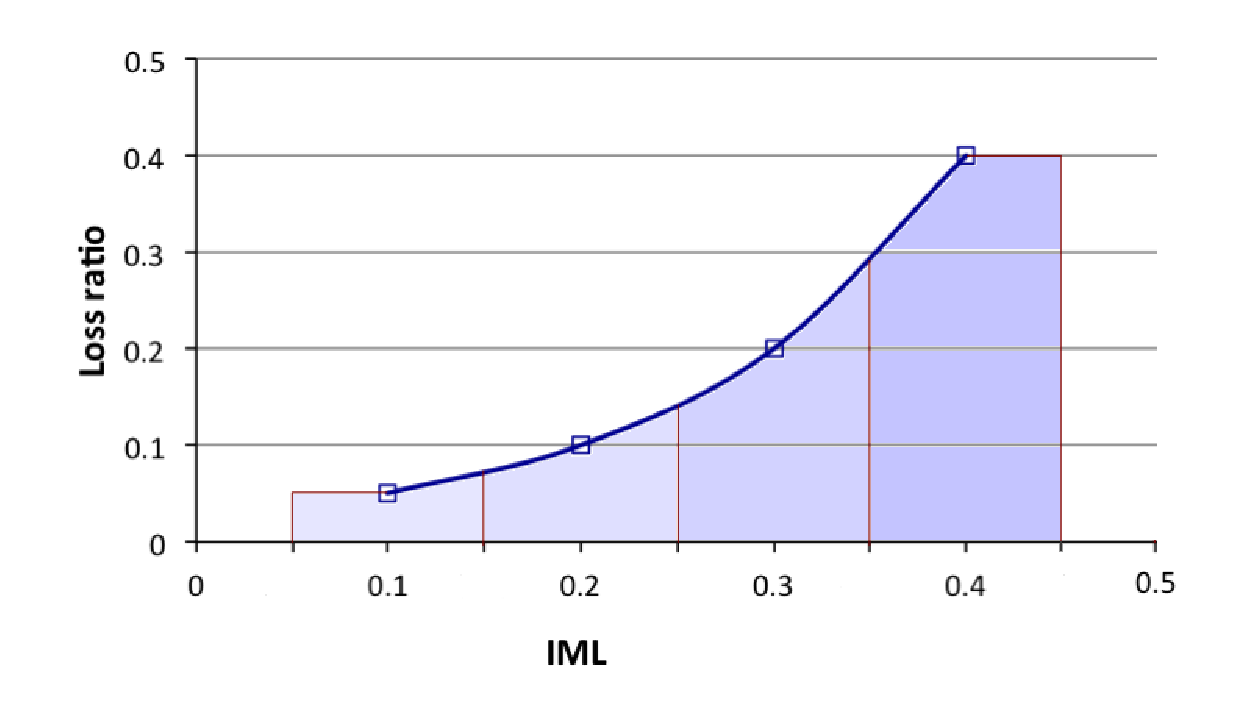
\includegraphics[width=8cm,height=5.5cm]{./Figures/Part_Risk/VF_intervals.eps}
\caption{Intervals for each intensity measure level on a discrete vulnerability function.}
\label{fig:VF_intervals}
\end{figure}

Note that for the first and last intensity measure level, there are no values before or after respectively. In this case, the lower and upper bound need to be computed based on the distance between the respective intensity measure level and the bound that was computed through one of the aforementioned formulae. Thus, the lower bound for the first intensity measure level can be given by:

\begin{equation}
Lower bound= IML_1-\frac{IML_2+IML_{1}}{2}
\end{equation}

And the upper bound for the last intensity measure level can be computed using:

\begin{equation}
Upper bound[IML_{n}]  = IML_{n}+\frac{IML_{n}-IML_{n-1}}{2}
\end{equation}

\item Once the intervals for each intensity measure level are defined, the probability of occurrence can be computed through the expression:

\begin{equation}
PO[IML_{n}]  = F(UB,\mu,\sigma)-F(LB,\mu,\sigma)
\end{equation}

Where $F$ stands for the cumulative distribution function, $UB$ and $LB$ stand for the upper and lower bound respectively of the $IML_n$ and $\mu$ and $\sigma$ stand for the logarithmic mean and standard deviation i.e. the mean ground motion and associated standard deviation of the normal distribution of the natural logarithm of the ground motion values.

\item Then, the mean loss ratio for each asset can be computed through the formula:

\begin{equation}
LR  = \sum_{n=1}^mPO[IML_n] \times LR_n
\end{equation}

\item The absolute mean loss can be computed by multiplying the mean loss ratio by the value of the asset contained on the exposure model file.

\end{enumerate}

To compute the standard deviation of the loss:

\begin{enumerate}
\item In order to compute this parameter, the total probability theorem needs to be used. The first step is to compute $E[LR_n^2]$, which is given by the following formula:

\begin{equation}
E[LR_n^2]=SD[LR_n]^2+E[LR_n]^2
\end{equation}

Where $SD[LR_n]$ stands for the standard deviation of the distribution of loss ratios and $E[LR_n]$ stands for the mean loss ratio.

\item Then, the total $E[LR^2]$ can be derived using the formula:

\begin{equation}
E[LR^2]=\sum_{n=1}^mPO[IML_n] \times E[LR_n]^2
\end{equation}

\item Subsequently the standard deviation of the loss ratio can be computed using the expression:

\begin{equation}
SD[LR]=\sqrt{E[LR^2]-E[LR]^2}
\end{equation}

Where $E[LR]$ stands for the mean loss ratio computed previously.

\item The absolute standard deviation of the loss can finally be computed by multiplying the standard deviation of the loss ratio by the value of the respective asset.

\end{enumerate}

\section{Method B}
\subsection{Description}
In this approach, for each ground motion field, the intensity measure level at a given site is used to calculate the mean and standard deviation of loss ratio using the vulnerability functions for each asset contained in the exposure file. Using these results, the mean and standard deviation of loss ratio across all events can be calculated. Again, loss ratios are converted into losses by multiplying by the value of the asset given in the exposure file. For this method, it is possible to aggregate the losses throughout the region and to compute the standard deviation of the aggregated loss. 

\subsection{Calculation workflow}

To compute the mean loss:

\begin{enumerate}
\item For each ground motion field, the intensity measure levels are related with the vulnerability functions to compute the mean loss ratio for each asset. Since currently the vulnerability functions are being defined in a discrete way, it is quite probable that the intensity measure level provided by the ground motion field is not contained in the vulnerability function. In these cases, linear interpolation methods are being employed to derive the mean loss ratio at the intensity measure level of interest.

\item The mean loss ratio for each asset across all possible simulations of the deterministic event can be calculated through the formula:

\begin{equation}
LR=\frac{\sum^m_{n=1}LR_n|IML}{m}
\end{equation}

Where $m$ stands for the number of ground motion fields simulated.

\item The mean loss can then be derived by multiplying the mean loss ratio by the value of the asset contained in the exposure model file.

\end{enumerate}

To compute the standard deviation of the loss:

\begin{enumerate}

\item Again, the total probability theorem is employed. $E[LR_n^2]$ is computed using the following formula:

\begin{equation}
E[LR_n^2]=SD[LR_n]^2+E[LR_n]^2
\end{equation}

Where $SD[LR_n]$ stands for the standard deviation of the distribution of loss ratios and $E[LR_n]$ stands for the mean loss ratio (for each ground motion field).

\item Then, the total $E[LR^2]$ can be derived using the formula:

\begin{equation}
E[LR^2]=\frac{\sum_{n=1}^m E[LR_n]^2}{m}
\end{equation}

\item The standard deviation of the loss ratio can be computed using the expression:

\begin{equation}
SD[LR]=\sqrt{E[LR^2]-E[LR]^2}
\end{equation}

Where $E[LR]$ stands for the mean loss ratio computed previously.

\item The standard deviation of the absolute loss can finally be computed by multiplying the standard deviation of the loss ratio by the value of the respective asset.

\end{enumerate}

